\pagestyle{plain}
\chapter{INTRODUCCIÓN}\label{cap:Introduccion}
%\vspace{0.2cm}
\noindent\rule{\linewidth}{1.3pt}\\
\startcontents[chapters]
\printcontents[chapters]{}{1}{}
\vspace{0.2cm}
\noindent\rule{\linewidth}{1.1pt}\\
%\minitoc
%\tableofcontents
\newpage

\section{Motivación}\label{sec:Motivacion}

\par En los últimos años la evolución del parque automovilístico español se ha decantado muy favorablemente hacia la tecnología diésel. Tal y como puede verse en la Figura \ref{fig:EvolucionParqueTurismos}, el número de turismos de motorización diésel matriculados en España desde 1998 ha sido superior al de turismos de motorización gasolina. La misma tendencia puede observarse para los demás tipos de vehículos. Este crecimiento es consecuencia de los avances tecnológicos en los motores diésel, que han consistido primordialmente en mejoras que disminuyen el consumo de combustible de estos motores con respecto a los motores de encendido provocado, con unas prestaciones similares y cumpliendo las exigencias tanto de los usuarios como de las cada vez más exigentes normativas sobre emisiones de partículas.

\begin{figure}[h]
\centering
	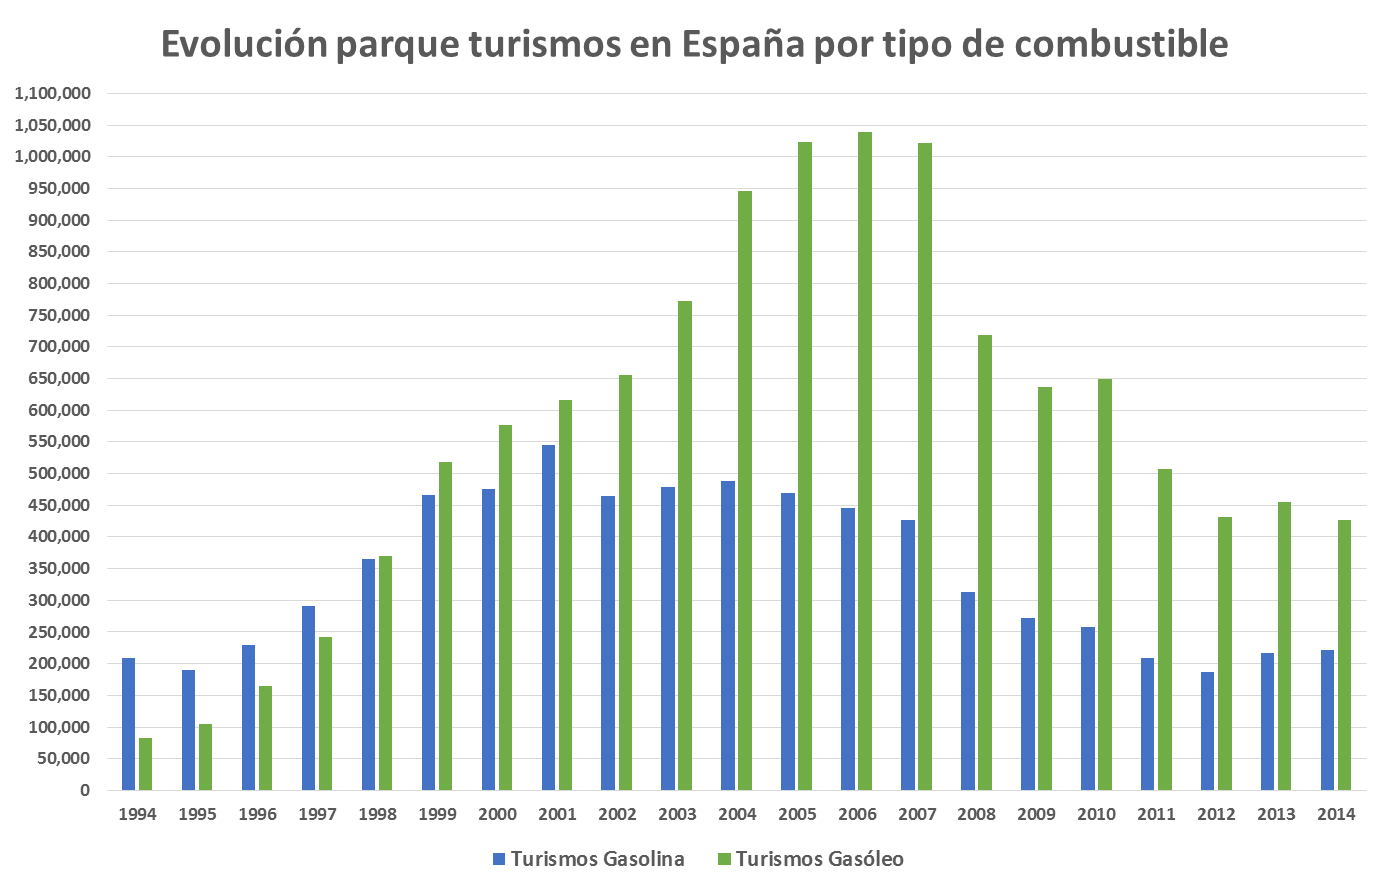
\includegraphics[width=0.6\textwidth]{Evolucionturismos.png}	 
	\caption[Evolución histórica de turismos diésel y gasolina en España]{Evolución parque turismos en España desde 1984 por motorización.\\ \textbf{Fuente:} \href{https://sedeapl.dgt.gob.es/IEST2/menu.do?path=/vehiculos/parque/&file=inebase&type=pcaxis&L=0&js=1}{Portal estadístico de la DGT}}	
\end{figure} \label{fig:EvolucionParqueTurismos}

\par Actualmente la protección del medio ambiente constituye una prioridad ineludible, particularmente en los países avanzados, aunque se ha extendido a la mayoría del resto de países con el Protocolo de Kyoto (1997) y con las cumbres mundiales de Clima, la última de las cuales se celebró en Nueva York (2014). Esta protección del medio ambiente se ha implementado mediante políticas ambientales que cada vez hacen las legislaciones más estrictas. En Europa actualmente están vigentes la Directiva 98/69/CE y la Directiva 2002/80/CE. En estas Normativas se establecen los valores límites para los motores de encendido por compresión ligeros. De las restricciones para los pesados se encarga la Directiva 2001/27/CE. Todas estas directivas establecen límites en términos de masa de partículas emitidas por kilómetro o por kWh.

\par Debido a esto, la mayoría de los estudios sobre emisiones de \index{partículas} partículas analizan exclusivamente los resultados de emisiones en masa. Sin embargo, también la \index{morfología} morfología de las partículas tiene gran importancia dada la notable influencia que ésta tiene sobre la salud humana y sobre el medio ambiente. Por tanto, además de regularse la masa de partículas emitida podría justificarse también algún tipo de regulación sobre el tamaño y la morfología de éstas. En concreto, la legislación medioambiental no es ajena a las normativas sobre el tamaño de las partículas y no es aventurado esperar que en el futuro alguna limitación del tamaño de las partículas se aplique también a las emisiones diésel. Más lejano aún y complejo resulta suponer, de momento, que otros aspectos de la morfología de las partículas puedan llegar a regularse.

\par Por otra parte, antes de ser expulsadas a la atmósfera, la morfología de las partículas tiene también un importante efecto sobre la eficiencia de retención de las \index{trampas de partículas} trampas de partículas, consideradas actualmente como uno de los sistemas de postratamiento necesarios en algunas estrategias de reducción de emisiones más interesantes de cara a cumplir las normativas de emisiones de los motores diésel.

\par Son precisamente los importantes efectos sobre la morfología de las partículas emitidas sobre los filtros de partículas, sobre la salud humana, sobre el medio ambiente y sobre el clima, los que justifican la realización de esta Tesis Doctoral, en línea con el creciente interés científico, como se demuestra en el estudio bibliométrico presentado en el apartado \ref{sec:Bibliometria}.

\section{Objetivos}\label{sec:Objetivos}

\par Principalmente, esta Tesis Doctoral se centra en tres objetivos, que son:

\begin{itemize}
	
	\item Estudio de cómo afecta la no esfericidad de la morfología de las partículas primarias a las características geométricas de los aglomerados diésel. En casi la totalidad de la literatura existente, se parte de la base de que los aglomerados están compuestos por partículas esféricas. Los efectos que pueden llevar a que las partículas no sean perfectamente esféricos son variados y pueden modelarse mediante un parámetro geométrico que permita determinar en qué cuantía la desviación de la idealidad esférica modifica los valores de la geometría fractal. Existen trabajos donde se han modelado estas geometrías, pero la manera en que afectan al prefactor y a la dimensión fractal está menos estudiado. Estos parámetros serán definidos en el capítulo \ref{cap:MetodosAnalisisFractal}. Partiendo de figuras que permiten imponer condiciones de contorno conocidas para dichos parámetros, es posible estudiar cómo se comportan éstos cuando la geometría de las partículas primarias se desvía de la esfericidad.
	
	\item Como se ha comentado anteriormente, para estudiar la geometría fractal de los aglomerados se han de asumir una serie de hipótesis que son aceptadas ampliamente en el ámbito de las emisiones de partículas diésel. Sin embargo, existen muy pocas referencias que cuestionen la validez de dichas hipótesis, o al menos, el rango de valores para los cuales su aplicabilidad está fuera de duda. Esta Tesis tiene como objetivo cuestionar algunas de estas hipótesis, entre ellas la hipótesis del número mínimo de partículas primarias para el cual un aglomerado puede ser considerado fractal o cuasi-fractal.
	
	\item Los fractales, como se expondrá a lo largo del Capítulo \ref{cap:MetodosAnalisisFractal} se encuentran en la naturaleza y es el lenguaje geométrico natural. Parece lógico que una metodología de análisis fractal aplicada al campo de emisiones pueda usarse sin muchas modificaciones a otros campos. Como ejemplo de ello, se aplicarán algunas técnicas a la caracterización fractal de rocas y fracturas hidráulicas usadas para la explotación de hidrocarburos.
	
	\item Con objeto de poder analizar una gran cantidad de parámetros y de morfologías para su posterior comparación, es necesario disponer de herramientas informáticas flexibles y desarrolladas \textit{ad hoc} para las aplicaciones objeto de interés de esta Tesis. Por ello, otro objetivo, aunque menor, de esta Tesis es la mejora y desarrollo de aplicaciones donde se implementen las metodologías desarrolladas en esta Tesis.
	
\end{itemize}

\par Para la consecución del primer objetivo se ha partido del enfoque geométrico seguido en la Tesis de Francisco Martos \cite{martosphD:2006} y en \cite{lapuertaetal:2006,lapuertaetal:2010}. A través de figuras geométricas cuya dimensión fractal es impuesta se pueden determinar el modelo matemático que siguen los parámetros a estudio y ver la influencia de la hipótesis de no esfericidad en la morfología de las partículas diésel. Para un estudio más pormenorizado se utilizó la herramienta informática que de desarrolló en el Proyecto Fin de Carrera \cite{vieraPFC:2014}. El uso de herramientas informáticas es de vital importancia para el estudio de la geometría de aglomerados bajo ciertas condiciones.

\par De igual modo, mediante el uso de otra herramienta informática \cite{delblancoPFC:2015} se puede analizar la dependencia de los resultados con respecto a una de las hipótesis impuestas en los modelos geométricos. Los aglomerados de partículas diésel son asimilados a figuras fractales cuando el número de partículas primarias es superior a cierto número, habiendo un consenso establecido para dicho número, pero sin una justificación lo suficientemente elaborada. La validez en el campo de las partículas diésel, donde los aglomerados tienen usualmente menos de doscientas ($n_{po}\,<\,200$) fue demostrado por \cite{megaridisetal:1990}. Después ha sido utilizado por numerosos autores para la caracterización de hollín \cite{zhuetal:2003,leeetal:2002,caietal:1995,gorbunovetal:1999,zuritaetal:2002,parketal:2004}.

\par El disponer de una metodología que sólo depende de la geometría y no del proceso que da origen a esa morfología, permite que las técnicas y herramientas desarrolladas en la presente Tesis puedan aplicarse a cualquier campo donde la naturaleza fractal de los fenómenos sea relevante.

\section{Antecedentes}\label{sec:Antecedentes}

\par El Grupo de Combustibles y Motores lleva estudiando las emisiones de los Motores diésel durante más de veinte años. Sus esfuerzos se han centrado en la caracterización de combustibles, tanto convencionales como alternativos. Cuando aún la tecnología de motores de encendido por compresión no había superado a la tecnología de los motores de encendido provocado, aunque estaba cerca de lograr este último hito, se presentó la Tesis de Rosario Ballesteros Yáñez \cite{chariphD:2002}. El trabajo de investigación que se presenta en su Tesis Doctoral se enmarca dentro del desarrollo y puesta a punto de herramientas de caracterización y análisis de partículas diésel. Además, los resultados experimentales obtenidos de ensayar combustibles de diferente origen y especificaciones permitieron mejorar el conocimiento que se poseía de los procesos que tienen lugar en el motor y que contribuyen a la generación y emisión de partículas diésel y ayudaron a establecer las directrices en cuanto a búsquedas de posibles nuevos combustibles de automoción y de soluciones óptimas en las que las prestaciones y las emisiones de los motores permaneciesen dentro de unos niveles adecuados. Este trabajo fue el primer estudio que se realizó sobre combustibles y emisiones de partículas diésel dentro de este grupo de investigación y constituyó un antecedente directo de otras Tesis Doctorales. 

\par Tal fue el caso de la Tesis de Francisco Javier Martos Ramos \cite{martosphD:2006}. Fue el primer trabajo dirigido hacia la caracterización morfológica de partículas mediante técnicas fractales. Se propone un método teórico-experimental para determinar los parámetros característicos, desde el punto de vista de la geometría fractal, de las emisiones provenientes de los motores diésel. Como continuación a esta Tesis Doctoral, José Martín Herreros Arellano \cite{martinphD:2009} centró su Tesis en estudiar el efecto del modo de funcionamiento y del combustible en la morfología de las partículas diésel. A partir de micrografías donde se estimaban el radio de giro y él área proyectada, se determinaban parámetros morfológicos de las partículas. Desde el punto de vista de emisiones, existen diferentes estrategias en cuanto a carga y regeneración de trampas de partículas. En este contexto, la Tesis de Fermín Olivas Miñana \cite{ferminphD:2012} se centró en caracterizar la influencia del combustible y de distintas condiciones operativas sobre el tamaño de las partículas, ampliando el estudio presentado en el artículo \cite{lapuertaetal:2007}.

\par Adicionalmente a estas Tesis, cabe mencionar el Proyecto Final de Carrera de Enrique Viera Luis \cite{vieraPFC:2014} que consistió en la implementación de una herramienta informática incluyendo el modelo propuesto en la Tesis de Francisco Javier Martos Ramos \cite{martosphD:2006}, ampliado en los artículos \cite{lapuertaetal:2010} y complementados por el Proyecto Final de Máster de Juan José Expósito González \cite{expositoPFM:2012}, corrigiendo algunas erratas en las ecuaciones de éste último. 

\par Los modelos empleados tienen hipótesis subyacentes que necesitan de herramientas matemáticas para su validación o para la limitación del rango de validez. En este sentido, el Trabajo Final de Grado de Marcos del Blanco Adán \cite{delblancoPFC:2015} desarrolla una metodología computacional ampliamente reconocida y aceptada en el campo de la geometría fractal.
\par El encuadre de la presente Tesis con referencia a los trabajos citados anteriomente se pueden ver en la Tabla.

\section{Metodología}\label{sec:Metodologia}

\par La metodología seguida en esta Tesis tiene un carácter eminentemente teórico. A partir de planteamientos matemáticos no excesivamente complejos se pretende ahondar en el conocimiento de aspectos morfológicos de agregados. Sin embargo, debido a que de abordan temas reales, no se descuida la aplicabilidad práctica de los resultados obtenidos. De igual forma se intentar maximizar las sinergias entre la práctica con la teoría, mediante las bases de datos de imágenes acumuladas desde hace años en el Grupo de Combustibles y Motores de la Universidad de Castilla-La Mancha.

\par La mayor parte de los ensayos se llevaron a cabo en las instalaciones de motores existentes en las Universidades de Castilla-La Mancha y de Málaga. Por un lado, en las primeras hay preparados para diferentes ensayos motores típicos de automoción de inyección directa completamente instrumentados con el triple objetivo de realizar medidas precisas, mantener el control de la instalación y asegurar la repetitividad de las condiciones de ensayo. En etas instalaciones experimentales hay disponibles técnicas experimentales de cierta complejidad que permiten la validación en tendencias de algunos resultados de los modelos planteados, así como otras técnicas experimentales menos complejas cuyos resultados alimentan a los modelos propuestos. Por otro lado, en las últimas hay disponibles técnicas experimentales correspondientes a la visualización de las partículas diésel y su posterior tratamiento digital. Los resultados de estas técnicas son de tipo geométrico y sus resultados son fundamentales para la entrada al modelo planteado sobre la morfología de partículas.

\par Con anterioridad e independencia a esta Tesis se obtuvieron una gran multitud de imágenes de aglomerados. Mediante técnicas de tratamiento de imágenes se pueden tratar para obtener parámetros geométricos característicos y usarlos para alimentar los modelos matemáticos de obtención de propiedades geométricas. Las interconexiones entre los métodos experimentales y teóricos se han esquematizado en la Figura.

\par La incorporación de técnicas de análisis de imágenes de tipo fractal ha permitido calcular la dimensión fractal de aglomerados de geometría conocida. Tal es el caso del método de Box-Counting que se explicará detalladamente en el Capítulo \ref{cap:MetodosAnalisisFractal}. Éste, junto con el resto de técnicas propuestas componen el conjunto de herramientas informáticas utilizadas.

\section{Bibliometría}\label{sec:Bibliometria}

\par Con el fin de demostrar la actualidad del interés de esta Tesis, se han realizado dos estudios bibliométricos, que se detallan en las Figuras y . Estos estudios bibliométricos se han realizado con el \emph{ISI Web of Knowledge} que tiene en su base de datos todas las publicaciones de interés internacional desde 1945.

\section{Viabilidad}\label{sec:Viabilidad}

\section{Desarrollo del Documento de la Tesis}\label{sec:DesarrolloDocumento}

\par La memoria de la presente Tesis Doctoral se compone de un total de nueve capítulos. En el primero de ellos se introduce y se justifica el porqué de la realización de este documento. Se hace una breve descripción de la historia y situación actual del grupo de investigación y se encuadra la Tesis Doctoral dentro de la línea de investigación. Igualmente, se expone la metodología seguida para la realización de la Tesis.

\par El segundo contiene una revisión del estado del arte en la morfología de las partículas en general, y específicamente sobre las partículas diésel. Inicialmente se hace una pequeña revisión a los distintos fenómenos de transporte a los que se pueden ver sometidas las partículas diésel, y que pueden dar lugar a distintos tipos de uniones. Una vez analizado cómo se conforman las partículas diésel desde su nucleación se comentan las distintas maneras de definir el tamaño de éstas y las funciones de distribución típicas. Posteriormente se describen los parámetros utilizados para definir las características morfológicas de las partículas. Se sigue con una descripción de geometrías fractales de campos distintos al de emisión de partículas en procesos de combustión. Finalmente, se comentan las implicaciones de la morfología y el tamaño de las partículas diésel sobre el medio ambiente y sobre la salud pública.

\par Dada la creciente importancia de los fractales en diversas aplicaciones, el capítulo tercero se centra en los métodos de análisis fractal desde un punto de vista puramente teórico. Se dan ejemplos de fractales conocidos y se hace un recorrido por esta incipiente rama de las matemáticas moderna, con reseñas históricas sobre sus principales contribuyentes. De carácter eminentemente teórico, es el capítulo más general de esta Tesis, aunque incluye aplicaciones a diversas ramas de la ingeniería. Una de ellas, las partículas diésel ocupa un apartado dentro de este capítulo. Se sigue con una descripción de otros fenómenos caracterizados por la geometría fractal, como son la caracterización de rocas y de dinámica de fluidos en medios porosos. Finalmente, se tocan otros temas adyacentes y que pretenden despertar la curiosidad de la aplicabilidad de las técnicas fractales como son el análisis de mercados y otras ramas del saber.

\par El cuarto capítulo es una particularización del tercero, centrándose en las partículas diésel. Se comienza dando unos conceptos básicos sobre los métodos geométricos de caracterización de partículas diésel mediante geometría fractal. Estos métodos se centran en la situación ideal de contacto puntual entre partículas. Posteriormente se describe el modelo empleado, desarrollando las ecuaciones matemáticas para los casos estudiados.

\par El quinto capítulo parte del modelo desarrollado en el capítulo anterior, relajando una de las hipótesis empleadas hasta ese capítulo. Se parte de partículas no esféricas, sino que están aplastadas. Primero se describen los procesos por los cuales la geometría de una partícula primaria podría no ser esférica. Después se define el parámetro físico para modelar esta geometría. Por último, se desarrollan las ecuaciones correspondientes y se compara con los resultados obtenidos en el capítulo cuarto.

\par En el sexto capítulo se realiza una crítica de las hipótesis del modelo. Se pretende comprobar la robustez de dichas hipótesis empleando diferentes herramientas matemáticas. Primero se introduce el método del Box-Counting que no depende de la geometría subyacente al problema. Se describe en qué consiste dicho modelo en primer lugar. Después, se aplica a figuras conocidas. Esto es necesario para comprobar la validez de este método. Dos hipótesis se ponen a prueba: la primera, la monodispersidad, es decir, la uniformidad en el tamaño de las partículas primarias que componen el aglomerado. La segunda y última, la esfericidad.

\par Como se ha comentado anteriormente, se dispone de una amplia base de datos con imágenes de aglomerados obtenidos en motores diésel, bien con combustible convencional o biocombustibles. Utilizando las herramientas presentadas en los capítulos anteriores, se pretende caracterizar la "huella" fractal de cada combustible. Para ello, los parámetros geométricos característicos juegan un papel determinante, como se verá en el Capítulo \ref{cap:AplicacionModelo}.

\par La Tesis termina con las conclusiones que se extraen a partir del trabajo realizado y sugerencias de trabajos futuros que se puedan derivar de lo desarrollado en esta Tesis.

\section{Resumen del Capítulo}\label{sec:ResumenCapitulo1}

\newpage
\bibliographystyle{Config/ealpha}	
\bibliography{Chapters/Bibliografia}